\section{Servicearchitektur}
In diesem Kapitel wird der Aufbau des Systems erläutert. 

\subsection{Vorteile der Microservice-Architektur im Vergleich zum Monolithen}

Die Microservice-Architektur stellt eine moderne Alternative zum klassischen monolithischen Architekturansatz dar. Bei einem Monolithen sind sämtliche Funktionalitäten der Anwendung innerhalb einer einzigen Codebasis und eines gemeinsam deployten Systems gebündelt. Änderungen an einzelnen Komponenten erfordern oftmals eine vollständige Neuveröffentlichung des Gesamtsystems, was zu hohen Wartungsaufwänden und eingeschränkter Flexibilität führt \cite{newman2021building}.

Im Gegensatz dazu ist die Microservice-Architektur durch eine feingranulare Zerlegung der Anwendung in unabhängige Dienste gekennzeichnet \cite{Dragoni2017}. Jeder dieser Dienste kapselt eine spezifische Funktionalität und kommuniziert über wohldefinierte Schnittstellen (z.B. REST oder Messaging-Systeme wie Solace).

Für das vorliegende System ergeben sich daraus mehrere konkrete Vorteile, die im Vergleich zur monolithischen Architektur besonders relevant sind. Im Bereich der Skalierbarkeit zeigt sich, dass einzelne Microservices – etwa die KI-Komponente oder der IoT-Dienst – unabhängig voneinander hoch- oder herunterskaliert werden können, ohne dass andere Systemteile betroffen sind. Dies ermöglicht eine ressourcenschonende und bedarfsgerechte Nutzung der Infrastruktur. Auch die Wartbarkeit des Systems profitiert erheblich vom modularen Aufbau: Fehlerbehebungen oder Erweiterungen können gezielt innerhalb einzelner Microservices erfolgen, ohne das Gesamtsystem zu beeinträchtigen. Dadurch verringert sich nicht nur das Risiko unerwünschter Nebeneffekte, sondern auch die Ausfallzeiten bei der Weiterentwicklung \cite{newman2021building}.

Darüber hinaus erlaubt die Microservice-Architektur eine differenzierte Ressourcenzuweisung. Dienste mit geringer Last können ressourcenschonend betrieben werden, was sich positiv auf die Betriebskosten auswirkt. Diese Effizienz ist bei monolithischen Systemen nur schwer zu erreichen, da dort stets das gesamte System bereitgestellt werden muss. Ein weiterer Vorteil liegt in der technologischen Vielfalt: Da Microservices entkoppelt sind, können unterschiedliche Programmiersprachen und Frameworks eingesetzt werden. So kann beispielsweise die KI-Analyse in Python erfolgen, während das Backend in Rust realisiert ist. Dies fördert die Nutzung spezialisierter Technologien je nach Anwendungsfall \cite{newman2021building}.

Nicht zuletzt verbessert sich durch Microservices auch die sogenannte Capability-Isolation. Bestimmte Verantwortlichkeiten – etwa die E-Mail-Verifikation oder die Steuerung der Hardware-Kommunikation – sind eindeutig lokalisiert und nur an einer Stelle im System implementiert. Dies erleichtert sowohl die Wartung als auch die gezielte Erweiterung einzelner Funktionen \cite{Dragoni2017}.

In Summe ergibt sich eine deutlich höhere Flexibilität, Erweiterbarkeit und Ausfallsicherheit. Für ein wachsendes System mit heterogenen Anforderungen – wie im vorliegenden Projekt – ist der Microservice-Ansatz daher der Monolith-Architektur in mehrfacher Hinsicht überlegen \cite{Dragoni2017}.

\begin{figure}[H]
	\centering
	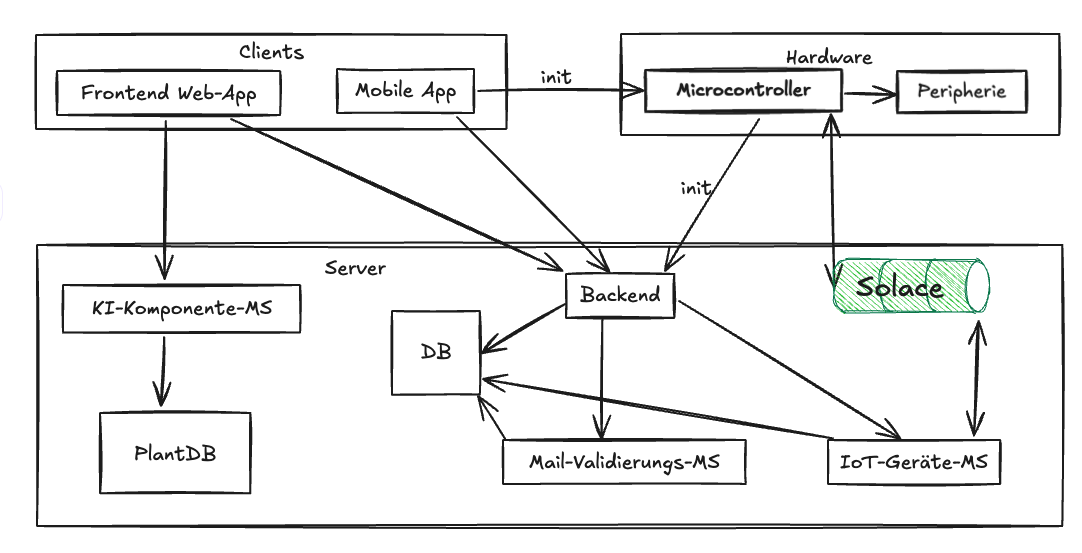
\includegraphics[scale=.35]{"./img/Kommunikation.png"}
	\caption{Kommunikation zwischen den Komponenten von Sensora}
	\label{fig:Kommunikation}
\end{figure}

\subsection{Hosting und Systemverbindungen}
Die Systemarchitektur der Anwendung basiert auf einem verteilten Ansatz, bei dem mehrere spezialisierte Komponenten zusammenwirken. Das Hosting erfolgt Docker basiert, wobei die Dienste in voneinander getrennten Containern betrieben werden. Diese Struktur ermöglicht eine hohe Skalierbarkeit und eine klare funktionale Trennung zwischen einzelnen Bereichen.
Zentraler Einstiegspunkt f"ur die NutzerInnen ist die Webanwendung bzw. die mobile App, welche beide als Client-Komponenten fungieren. Gew"ohnlich verl"aufen alle Anfragen dieser Clients über das zentrale Backend. Dieses bildet den Kern der Serverarchitektur und übernimmt die Koordination aller systemrelevanten Prozesse.
Eine Besonderheit stellt das Hinzufügen neuer Controller dar. In diesem Fall kommuniziert der Client direkt mit dem Mikrocontroller, um eine initiale Verbindung und Konfiguration zu ermöglichen. Diese Kommunikation ist notwendig, um die Geräte korrekt in das System einzubinden, bevor sie in den regulären Datenfluss übergehen.
Einige Komponenten wurden bewusst aus dem Haupt-Backend ausgelagert, um Zuständigkeiten zu trennen und das System modular zu halten. Dazu gehört unter anderem die Kommunikation mit den Mikrocontrollern, die über eine eventbasierte Architektur mithilfe des Nachrichtensystems \textit{Solace} realisiert wird. Dabei senden die Controller ihre Sensordaten nicht direkt an das Backend, sondern publizieren diese über Solace. Ein spezialisierter Microservice nimmt diese Nachrichten entgegen und verarbeitet sie asynchron weiter.
Auch die E-Mail-Verifikation sowie die Analyse durch die KI-Komponente sind eigenständige Microservices, die über interne APIs in das Gesamtsystem integriert sind. Dies erlaubt eine unabhängige Entwicklung und Wartung dieser Teilfunktionen ohne direkte Abhängigkeit vom Kernsystem.
Die Datenpersistenz erfolgt über eine zentrale Datenbank, welche alle benutzerbezogenen und systemkritischen Informationen verwaltet. Die KI-Komponente nutzt für ihre Analysen eine separate Datenbasis zur Speicherung pflanzenspezifischer Informationen.
Insgesamt ergibt sich ein flexibles, erweiterbares System, das sowohl unmittelbare Benutzerinteraktionen als auch zeitlich versetzte, datengesteuerte Prozesse unterstützt.
